\documentclass[../main.tex]{subfiles}

\begin{document}

\chapter{Об’єктно-орієнтоване проектування ІС}

Якщо аналіз об’єкта проектування – це розробка відповідної логічної моделі, яка описує усі можливі та прийнятні варіанти розв’язання задач, які вказують, що повинна робити система, то проектування – це вироблення рішення відповідно до моделі аналізу, яке оптимізує набір критеріїв проектування, які  показують, як ця поведінка (робота) системи може бути реалізована \cite{diploma_guidelines}.
Оскільки, у даній роботі застосовується об’єктно-орієнтована технологія проектування, то проектна частина повинна складатися із таких етапів:

\begin{enumerate}
	\item Архітектурне проектування – описує логічну структуру інформаційної системи (програмні класи, підсистеми,  пакети) та їх зв’язки.
	\item Детальне проектування – описує структури даних та алгоритми всередині окремих класів. 
\end{enumerate}

\section{Архітектурне проектування}
Формування архітектури – перший і основний крок у розв’язанні завдання проектування, що закладає фундамент уявлення програмної системи, здатної виконувати весь спектр детальних вимог. \cite{diploma_guidelines2}

Створення архітектури – це проектування на найвищому рівні (логічна архітектура). Логічна архітектура описує систему в термінах її принципової організації у вигляді пакетів, програмних класів і підсистем. Вона називається логічною, оскільки не визначає способи розгортання цих елементів у різних операційних системах або на фізичних комп’ютерах в мережі (це відноситься до архітектури розгортання) \cite{diploma_guidelines}.

Програмий додаток для операційної системи Android складається з набору активностей (activity), кожній з яких відповідає вікно додатку. Кожна активність представлена в проекті класом, що реалізований на мові Java та зберігається в однойменному файлі з розширенням .java. Кожній активності відповідає xml файл-опис. В xml-файлі описано розташування об'єктів, що візуалізуються. При запуску активності система Android автоматично розпізнає розмір екрану мобільного пристрою і приводить контент у відповідність з розміткою, описаної в xml-файлі. Таким чином, одна і та ж активність буде виглядати однаково незалежно від діагоналі пристрою, що використовується. 

Також, для кожного Android-додатку повинен існувати xml-файл, так званий маніфест (AndroidManifest), в якому будуть прописані мінімальні вимоги до системи, всі активності додатку, сервіси та дозволи, які потрібні додатку для функціонування \cite{pro_android}.

Одним з важливих етапів архітектурного проектування є побудова діаграми пакетів. Діаграма пакетів є діаграмою, яка містить пакети класів і залежності між ними. Вона описує архітектурну основу системи і допомагає в управлінні масштабами і складністю системи. Діаграма пакетів для додатку зображена на рис. \ref{diagram:packages}.
\vspace{\baselineskip}

\begin{figure}[H]
	\centering
	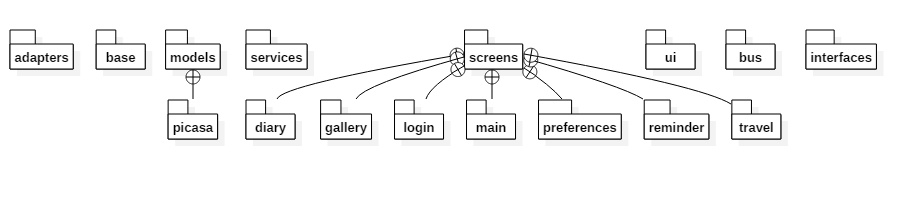
\includegraphics[width=1\textwidth]{diagram_packages}
	\caption{Діаграма пакетів для Android-щоденника}
	\label{diagram:packages}
\end{figure}

Пакет \textit{\textbf{adapters}} призначений для адаптерів. Адаптер -- це об'єкт, що діє як міст між предсталенням (view) і даними для цього представлення. Він забезпечує доступ до елементів даних. Також, адаптер відповідальний за подання представлення для кожного елемента в наборі даних \cite{adapter}. 

В пакеті \textit{\textbf{models}} будуть знаходитися класи моделей, що необхідні для взаємодії з базою даних чи іншими сервісами. Пакет \textit{\textbf{screens}} призначений для класів активностей, що являють собою окремі екрани додатку, тому в нього були додані додаткові пакети, щоб розділити екрани по областях, за які вони відповідають.

Пакет \textit{\textbf{services}} буде містити сервіси. В Android сервіс (або служба) -- це компонент додатку, котрий може виконувати	довготривалі операції в фоновому режимі і не містить користувацького інтерфейсу.

Ще одним будівельним блоком для створення архітектури об'єктно-орієнтованої системи вважається компонент. Діаграма компонентів показує розбиття програмної системи на структурні компоненти та залежності між компонентами. В якості фізичних компонентів можуть бути файли, бібліотеки, модулі, виконувані файли, пакети і т.п. У багатьох середовищах розробки модуль або компонент відповідає файлу. Стрілки, що з'єднують модулі, показують відносини взаємозалежності аналогічні тим, які мають місце при компіляції вихідних текстів програм. Основними графічними елементами діаграми компонентів є компоненти, інтерфейси і залежності між ними. 

Діаграму компонентів для Android-щоденника зображено на рис. \ref{diagram:hierarchy}.

%TODO: describe this

\begin{figure}[H]
	\centering
	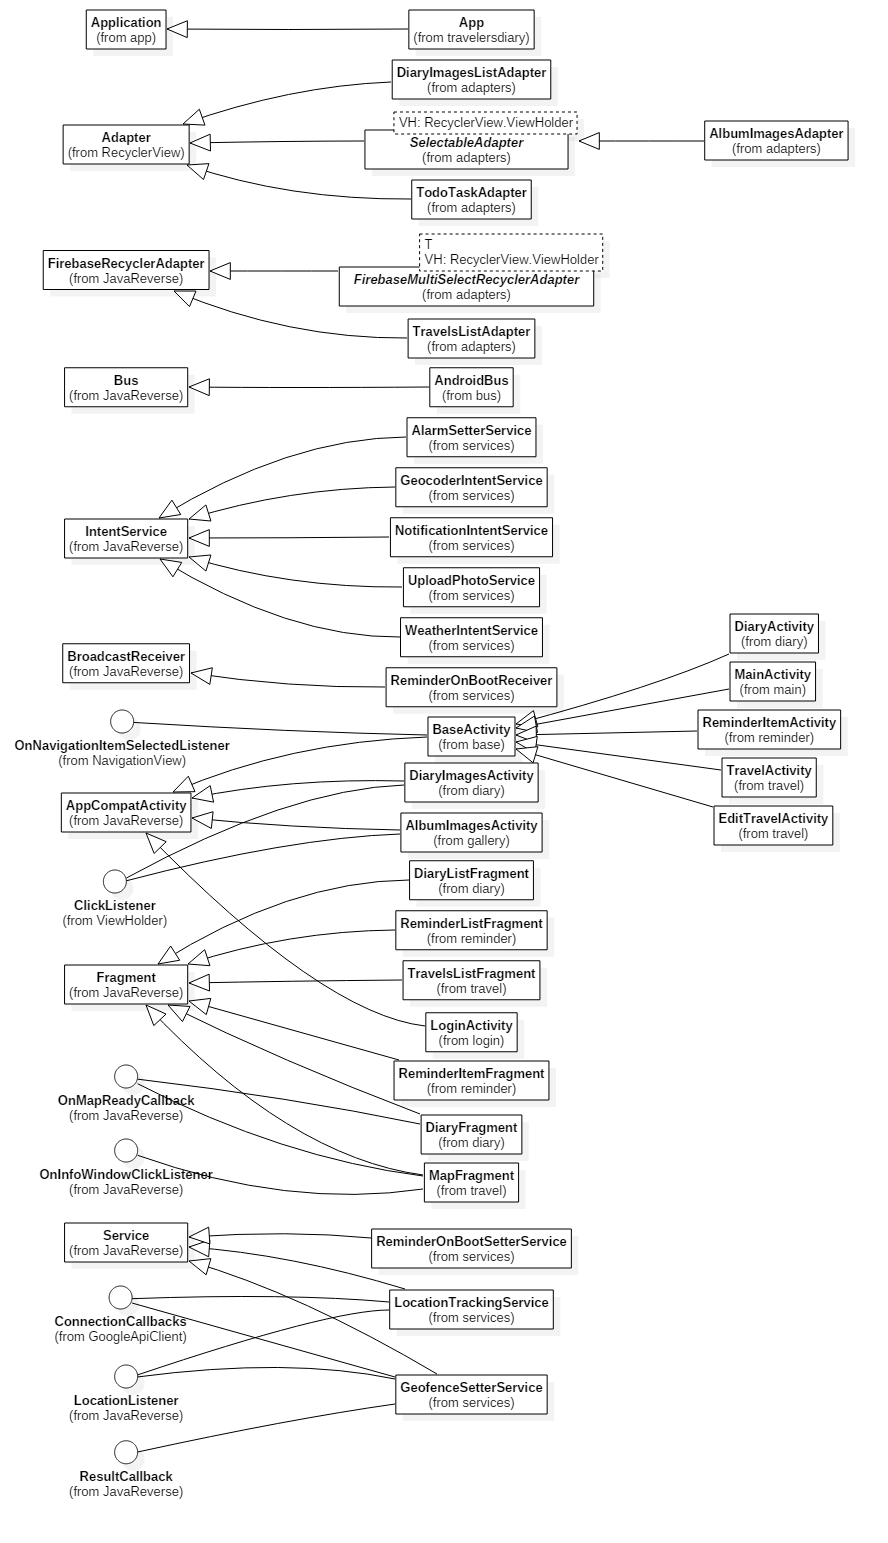
\includegraphics[height=0.8\textheight]{diagram_hierarchy}
	\caption{Діаграма компонентів Android-щоденника}
	\label{diagram:hierarchy}
\end{figure}

\section{Детальне проектування}

Детальне проектування – описує структури даних та алгоритми всередині окремих класів [10]. 

У програмуванні структури даних ‒ це способи організації даних в комп’ютерах. Часто разом зі структурою даних пов’язується і специфічний перелік операцій, які можуть бути виконаними над даними.
Правильний підбір структур даних є надзвичайно важливим для ефективного функціонування відповідних алгоритмів їх обробки. Добре побудовані структури даних дозволяють оптимізувати використання машинного часу та пам’ятті комп’ютера для виконання найбільш критичних операцій.

Логічна будова інформаційної системи (див. рис. \ref{diagram:models}) побудована  за допомогою UML-діаграми класів, яка служить для представлення статичної структури моделі системи в термінології класів об’єктно-орієнтованого програмування.

\begin{figure}[H]
	\centering
	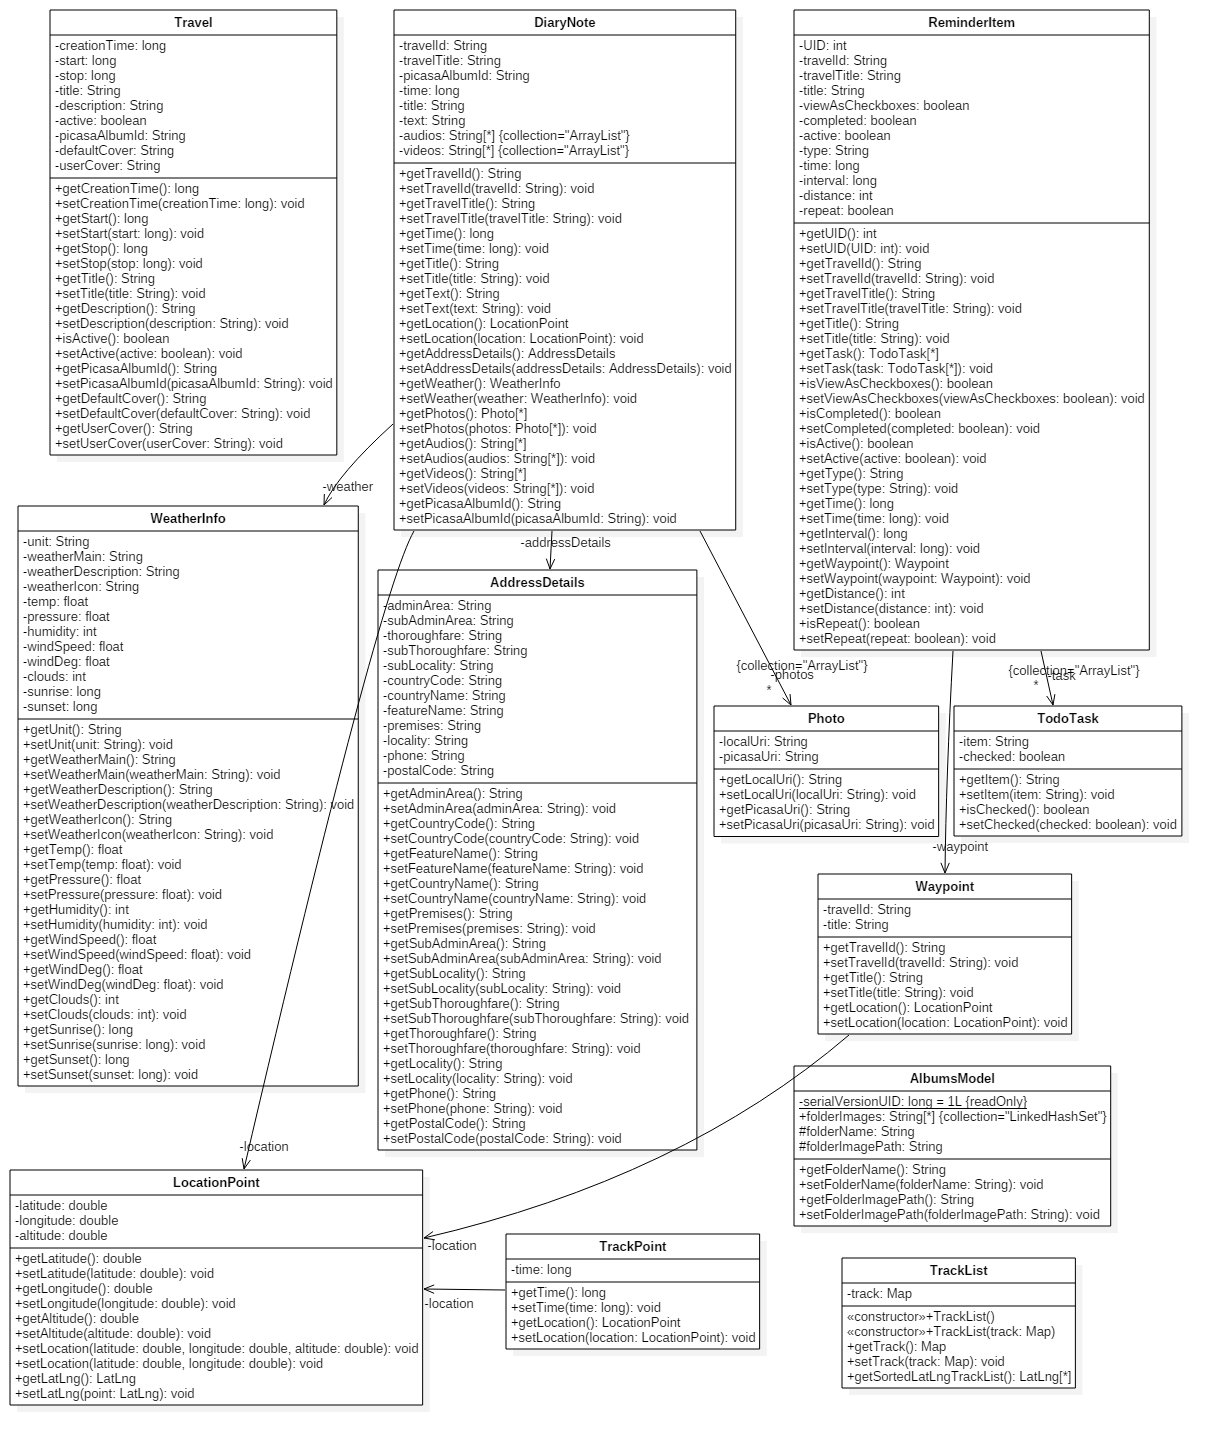
\includegraphics[height=0.8\textheight]{diagram_models}
	\caption{Діаграма моделей Android-щоденника}
	\label{diagram:models}
\end{figure}

Дані моделі використовуються для збереження об'єктів до бази даних та їх отримання.

%TODO: add models description

\section{Розгортання програмної системи на апаратних засобах}

Для функціонування додатку необхідна операційна система Android версії 4.2 (API 16) і вище.

%TODO: add something here

\section{Висновки}

%TODO: Висновки до розділу (не більш 1-2 сторінки). Розмір одного висновку приблизно – один абзац (5-7 рядків). Висновки цього розділу є важливою і значущою частиною роботи.

\end{document}